
%(BEGIN_QUESTION)
% Copyright 2008, Tony R. Kuphaldt, released under the Creative Commons Attribution License (v 1.0)
% This means you may do almost anything with this work of mine, so long as you give me proper credit

The equation for voltage gain ($A_V$) in a typical noninverting, single-ended opamp circuit is as follows:

$$A_V = {R_{1} \over R_{2}} + 1$$

\noindent
Where,

$R_1$ is the feedback resistor (connecting the output to the inverting input)

$R_2$ is the other resistor (connecting the inverting input to ground)

\vskip 10pt

Suppose we wished to change the voltage gain in the following circuit from 5 to 6.8, but only had the freedom to alter the resistance of $R_{2}$:

$$\includegraphics[width=15.5cm]{i03264x01.eps}$$

Algebraically manipulate the gain equation to solve for $R_2$, then determine the necessary value of $R_2$ in this circuit to give it a voltage gain of 6.8.

\underbar{file i03264}
%(END_QUESTION)





%(BEGIN_ANSWER)

$$R_2 = {R_1 \over {A_V - 1}}$$

\vskip 10pt

For the circuit shown, $R_2$ would have to be set equal to 810.3 $\Omega$.

%(END_ANSWER)





%(BEGIN_NOTES)

Nothing more than a little algebra to obtain the answers for this question!

%INDEX% Electronics review: opamp noninverting amplifier circuit

%(END_NOTES)


